The raw spectrum of $^{133}$Ba is depicted in Figure \ref{fig:raw_data}.

\begin{figure}[H]
\centering
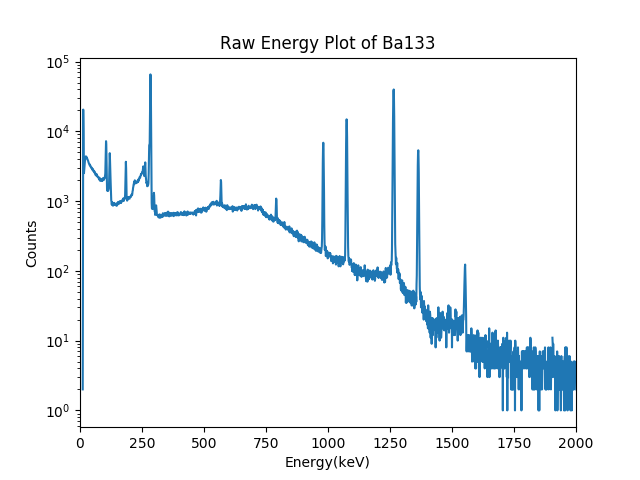
\includegraphics[scale=0.8]{images/Raw_spectrum.png}
\caption{Raw data of $^{133}$Ba produced from a HPGe detector.}
\label{fig:raw_data}
\end{figure}

Inspection of Figure \ref{fig:raw_data} shows that the data has not been calibrated yet.
For this analysis, I used 5 peaks from $^{133}$Ba
detailed in \ref{table:energy} \cite{Untitled27:online}.

\begin{table}[H]
\caption{$^{133}$Ba Gamma-ray Energies}
\begin{center}
\begin{tabular}{|l|c|c|r|}
\textbf{Source} & \textbf{Energy (keV)}\\
\hline
$^{133}$Ba    &  80.9979 \\
              &  276.3989 \\
              & 302.8508  \\
              & 356.0129 \\
              & 383.8485 \\
\hline
\end{tabular}
\end{center}
\label{table:energy}
\end{table}

I excluded 79.6142 keV from the energy list because it blurs together with
80.99 keV into one photopeak due to the energy resolution
of the HPGe. A better resolution detector would be needed to distinguish
these two peaks. Thus, I removed it so the iterator in the program will
not search for a peak that is not present.

After performing the linear calibration with $^{137}$Cs and $^{241}$Am,
a slope-intercept was found.
\vspace{5mm} %5mm vertical space
\begin{equation}
E = 0.28054*x + 1.26023
\end{equation}
\vspace{5mm} %5mm vertical space

The slope and intercept was applied to the channel number of the raw Ba133 data.
Figure \ref{fig:CE} depicts the two-point calibration.

\begin{figure}[H]
\centering
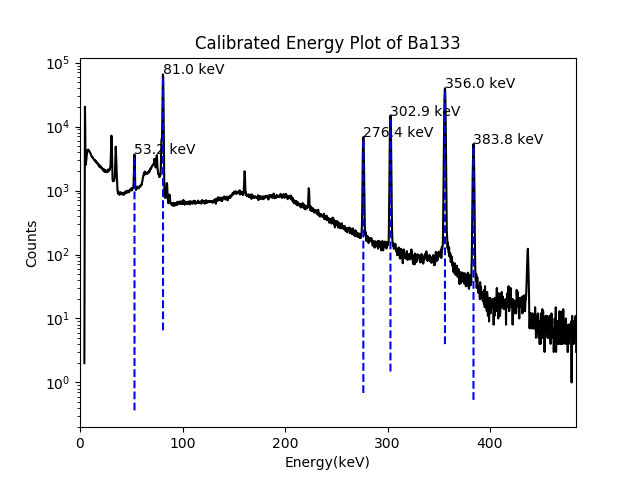
\includegraphics[scale=0.8]{images/Ba133_calibrated.png}
\caption{Calibrated $^{133}$Ba data with their corresponding gamma-ray energies
depicted by dashed blue lines}
\label{fig:CE}
\end{figure}

The difference between the calibrated peak locations and the expected peak
are shown in Table \ref{table:difference}.

\begin{table}[H]
\caption{$^{133}$Ba Gamma-ray Energies}
\begin{center}
\begin{tabular}{|l|c|c|r|}
\textbf{Source} & \textbf{Energy (keV)} & \textbf{Calibrated Energy} & \textbf{Difference (\%)}\\
\hline
$^{133}$Ba    &  80.9979 +/- 0.0011  & 81.0231 +/- 0.02546 & 0.03108 +/- 0.03147 \\
              &  276.3989 +/- 0.0012 & 276.4462 +/- 0.0053907 & 0.017148 +/- 0.001998 \\
              & 302.8508 +/- 0.0005 & 302.8877 +/- 0.008467 & 0.01217 +/- 0.0028006  \\
              & 356.0129 +/- 0.0007 & 356.038 +/- 0.006710 & 0.0070492 +/- 0.001895 \\
              & 383.8485 +/- 0.0012 & 383.8706 +/- 0.009235 & 0.005751 +/- 0.0024263 \\
\hline
\end{tabular}
\end{center}
\label{table:difference}
\end{table}

Based on Table \ref{table:difference}, the percent difference between the actual peak energies
and the calibrated spectrum is minute, which would be expected since semiconductors are nearly
linear with energy.
